\definecolor{ncp} {RGB}{191,255,191}
\definecolor{car} {RGB}{255,191,255}
\definecolor{bike}{RGB}{255,255,191}
\begin{figure}[h]
  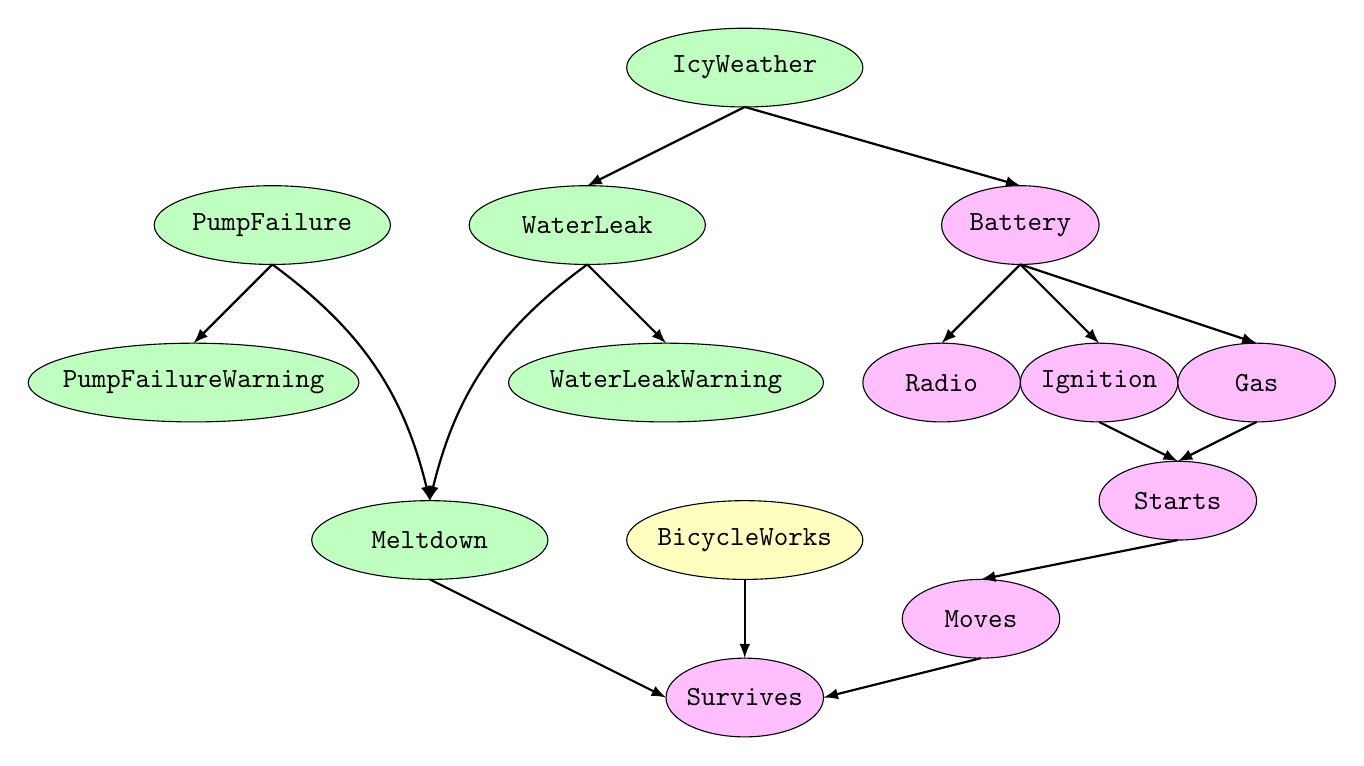
\begin{tikzpicture}

    \draw[fill=ncp] (7,9) ellipse (1.5cm and .5cm) node(a){\texttt{IcyWeather}};
    \draw[fill=ncp] (5,7) ellipse (1.5cm and .5cm) node(b){\texttt{WaterLeak}};
    \draw[fill=ncp] (1,7) ellipse (1.5cm and .5cm) node(c){\texttt{PumpFailure}};
    \draw[fill=ncp] (0,5) ellipse (2.1cm and .5cm) node(d){\texttt{PumpFailureWarning}};
    \draw[fill=ncp] (6,5) ellipse (2cm and .5cm) node(e){\texttt{WaterLeakWarning}};
    \draw[fill=ncp] (3,3) ellipse (1.5cm and .5cm) node(f){\texttt{Meltdown}};
    
    \draw[fill=car] (10.5,7) ellipse (1cm and .5cm) node(g){\texttt{Battery}};
    \draw[fill=car] (9.5,5) ellipse (1cm and .5cm) node(h){\texttt{Radio}};
    \draw[fill=car] (11.5,5) ellipse (1cm and .5cm) node(i){\texttt{Ignition}};
    \draw[fill=car] (13.5,5) ellipse (1cm and .5cm) node(j){\texttt{Gas}};
    \draw[fill=car] (12.5,3.5) ellipse (1cm and .5cm) node(k){\texttt{Starts}};
    \draw[fill=car] (10,2) ellipse (1cm and .5cm) node(l){\texttt{Moves}};
    \draw[fill=car] (7,1) ellipse (1cm and .5cm) node(m){\texttt{Survives}};

    \draw[fill=bike] (7,3) ellipse (1.5cm and .5cm) node(){\texttt{BicycleWorks}};

    \draw[arrows={-latex},thick] (7,8.5) to (5,7.5);
    \draw[arrows={-latex},thick] (5,6.5) to (6,5.5);
    \draw[arrows={-latex},thick] (5,6.5) to [bend right=20] (3,3.5);
    \draw[arrows={-latex},thick] (1,6.5) to (0,5.5);
    \draw[arrows={-latex},thick] (1,6.5) to [bend left=20] (3,3.5);
    \draw[arrows={-latex},thick] (3,2.5) to (6,1);

    \draw[arrows={-latex},thick] (7,8.5) to (10.5,7.5);
    \draw[arrows={-latex},thick] (10.5,6.5) to ( 9.5,5.5);
    \draw[arrows={-latex},thick] (10.5,6.5) to (11.5,5.5);
    \draw[arrows={-latex},thick] (10.5,6.5) to (13.5,5.5);
    \draw[arrows={-latex},thick] (11.5,4.5) to (12.5,4);
    \draw[arrows={-latex},thick] (13.5,4.5) to (12.5,4);
    \draw[arrows={-latex},thick] (12.5,3) to (10,2.5);
    \draw[arrows={-latex},thick] (10,1.5) to (8,1);

    \draw[arrows={-latex},thick] (7,2.5) to (7,1.5);

  \end{tikzpicture}
  \caption{Bayesian network for survival probability in regards of vehicle and powerplant status.}
  \label{figcar}
\end{figure}
